\documentclass[12pt,a4paper]{article}
\usepackage{amsmath,amssymb}
\usepackage{graphicx}
\usepackage{listings}
\usepackage{xcolor}
\usepackage{geometry}
\usepackage{subcaption}
\geometry{margin=2.5cm}

% --- تنظیمات نمایش کدها (Listings) ---
\lstset{
    basicstyle=\small\ttfamily,
    backgroundcolor=\color{gray!10},
    frame=single,
    breaklines=true,
    postbreak=\mbox{\textcolor{red}{$\hookrightarrow$}\space},
    keywordstyle=\color{blue}\bfseries,
    commentstyle=\color{green!60!black},
    stringstyle=\color{purple},
    showstringspaces=false,
    columns=fullflexible,
    keepspaces=true
}

% --- تنظیمات هایپرلینک ---
\usepackage{hyperref}
\hypersetup{
    colorlinks=true,
    linkcolor=blue,
    urlcolor=cyan
}

% --- تنظیمات زی‌پرشین (باید آخرین پکیج لود شود) ---
\usepackage{xepersian}

% تنظیم فونت‌ها (فونت‌های استاندارد موجود در Overleaf)
\settextfont{Amiri}
\setlatintextfont{Noto Sans}

\title{\textbf{گزارش جامع راه‌اندازی سخت‌افزاری و مش‌بندی گره‌های ESP32 در پلتفرم RuView (WiFi-DensePose)}}
\author{امیرعلی یزدانی}
\date{\today}

\begin{document}

\maketitle
\tableofcontents
\newpage

\section{مقدمه و هدف پروژه}
هدف از این پروژه، پیاده‌سازی و راه‌اندازی سیستم حسگری مبتنی بر سیگنال‌های وای‌فای (\lr{WiFi CSI Sensing}) با استفاده از پلتفرم متن‌باز \lr{RuView} و گره‌های سخت‌افزاری \lr{ESP32-S3} است. در این فرآیند، استخراج اطلاعات وضعیت کانال (\lr{Channel State Information}) جهت پایش حضور، تحرک، تنفس و بازسازی فضایی چندگره‌ای (\lr{Multi-Static Mesh}) به‌صورت بی‌درنگ انجام گرفته است.

\section{آماده‌سازی محیط توسعه و نصب ESP-IDF}
در ابتدای کار، برای سازگاری کامل با فریم‌ورک سورس‌کد \lr{RuView} و معماری چیپ \lr{ESP32-S3}، نسخه پایدار \textbf{\lr{ESP-IDF v5.4}} نصب گردید.

\subsection{نصب پیش‌نیازهای سیستمی اوبونتو}
ابتدا پکیج‌های پایه و ابزارهای بیلد در لینوکس اوبونتو نصب شدند:

\begin{latin}
\begin{lstlisting}[language=bash]
sudo apt-get update
sudo apt-get install -y git wget flex bison gperf python3 python3-pip python3-venv \
    cmake ninja-build ccache libffi-dev libssl-dev dfu-util libusb-1.0-0
\end{lstlisting}
\end{latin}

\subsection{کلون و نصب نسخه v5.4}
نسخه ۵.۴ فریم‌ورک به شکل بازگشتی کلون و کامپایلر ابزارهای تارگت \lr{esp32s3} نصب شد:

\begin{latin}
\begin{lstlisting}[language=bash]
mkdir -p ~/esp
cd ~/esp
git clone -b v5.4 --recursive https://github.com/espressif/esp-idf.git
cd esp-idf
./install.sh esp32s3
\end{lstlisting}
\end{latin}

نکته ای که اینجا حتما باید به آن توجه شود این است که توی داکیومنت اصلی به اشتباه نوشته شده v5.2 
ولی این ورژن مشکل های جدی دارد که قابل استفاده نیست.

\section{مراحل پیکربندی و فلش فریم‌ورک روی بردهای ESP32-S3}
برای برنامه‌ریزی هر یک از بردها، مراحل زیر به ترتیب اجرا شدند:

\subsection{لود متغیرهای محیطی و تعیین پورت}
قبل از هر کار، متغیرهای محیطی فعال شده و دسترسی کامل به پورت سریال داده شد:

باید پورتی که esp32
به آن متصل شده را در بیاریم به طور مثال در این مثال به پورت ttyACM0
متصل شده است.

\begin{latin}
\begin{lstlisting}[language=bash]
. $HOME/esp/esp-idf/export.sh
sudo chmod 666 /dev/ttyACM0
cd ~/Desktop/Amirali/WifiSensing/ruview/firmware/esp32-csi-node
\end{lstlisting}
\end{latin}

\subsection{تنظیمات معماری و پیکربندی شبکه (menuconfig)}
ابتدا چیپ تارگت روی \lr{esp32s3} تنظیم شده و منوی پیکربندی باز شد:

\begin{latin}
\begin{lstlisting}[language=bash]
idf.py set-target esp32s3
idf.py menuconfig
\end{lstlisting}
\end{latin}

در محیط متنی منو، وارد مسیر زیر شدیم:
\begin{center}
\textbf{\lr{Component config} $\rightarrow$ \lr{CSI Node Configuration}}
\end{center}

پارامترهای زیر با دقت مقداردهی شدند:
\begin{itemize}
    \item \textbf{\lr{WiFi SSID}:} نام شبکه وای‌فای محیط (\lr{Sharif-WiFi})
    \item \textbf{\lr{WiFi Password}:} برای شبکه‌های باز خالی گذاشته شد.
    \item \textbf{\lr{Aggregator IP}:} آدرس آی‌پی لپ‌تاپ در شبکه مشترک (به‌عنوان مثال: \lr{172.27.2.87})
    \item \textbf{\lr{Aggregator Port}:} مقدار پیش‌فرض پورت \lr{UDP} روی \textbf{۵۰۰۵}
    \item \textbf{\lr{Node ID (0-255)}:} شناسه یکتای هر برد 
\end{itemize}

\begin{figure}[htbp]
    \centering
    % تصویر سمت راست (در زبان فارسی زیرنویس الف به عنوان تصویر اول)
    \begin{subfigure}[b]{0.48\textwidth}
        \centering
        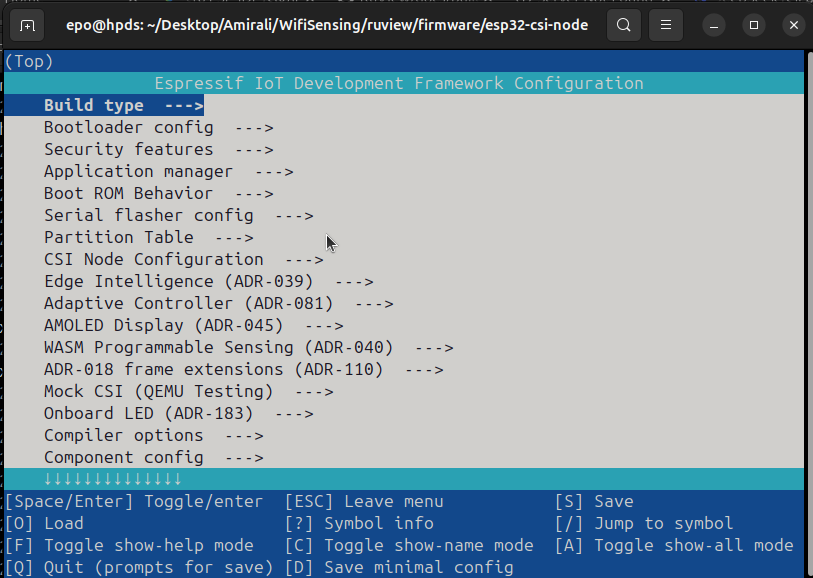
\includegraphics[width=\linewidth]{ImagesPhase2/menuconfig1.png}
        \caption{منوی اصلی ESP-IDF}
        \label{fig:menu_main}
    \end{subfigure}
    \hfill
    % تصویر سمت چپ (زیرنویس ب)
    \begin{subfigure}[b]{0.48\textwidth}
        \centering
        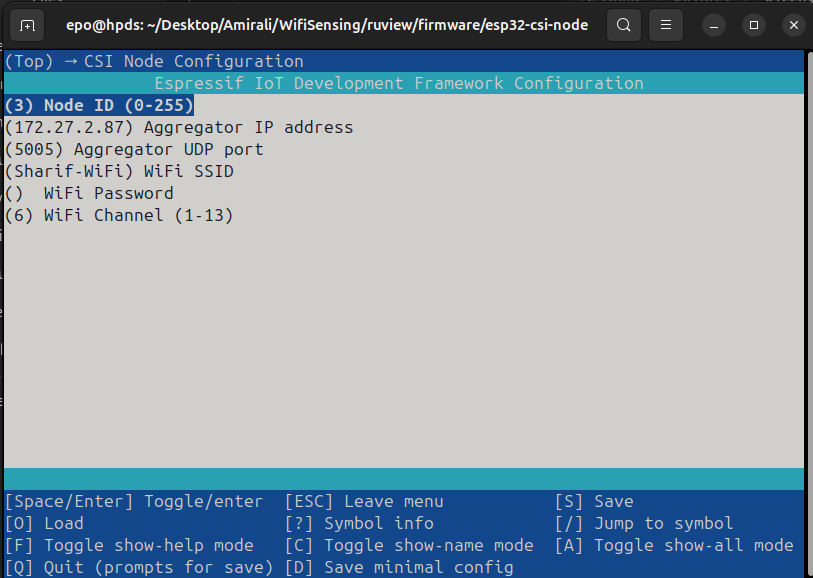
\includegraphics[width=\linewidth]{ImagesPhase2/menuconfig2.png}
        \caption{منوی پیکربندی پارامترهای گره CSI}
        \label{fig:menu_csi_node}
    \end{subfigure}
    
    \caption{محیط تنظیمات menuconfig: (الف) منوی اصلی و (ب) منوی تنظیم مشخصات وای‌فای و شناسه گره}
    \label{fig:menuconfig_comparison}
\end{figure}

\subsection{پاک‌سازی حافظه قبلی، فلش و راه‌اندازی}
برای جلوگیری از تداخل فریم‌ورک‌های قبلی، حافظه فلش پاک و کد جدید تزریق شد:

\begin{latin}
\begin{lstlisting}[language=bash]
idf.py -p /dev/ttyACM0 erase-flash
idf.py -p /dev/ttyACM0 flash monitor
\end{lstlisting}
\end{latin}

\paragraph{نکته مهم سخت‌افزاری:} پس از اتمام فلش، برای رفع باگ لایه فیزیکی \lr{Native USB CDC} و آغاز بی‌درنگ اتصال وای‌فای، دکمه سخت‌افزاری \textbf{\lr{RST / EN}} روی برد فشرده شد که منجر به سفید شدن ال‌ای‌دی وضعیت گردید.


\section{راه‌اندازی سرور پردازش حسگری \lr{(Sensing Server)} و داشبورد تحت وب}
پس از اتمام فلش و روشن شدن گره‌ها، هستهٔ سرور پردازش و ادغام داده‌ها (\lr{sensing-server}) که با زبان \lr{Rust} و فریم‌ورک وب \lr{Axum} توسعه داده شده است، اجرا گردید.

\subsection{دستور اجرای سرور در حالت سخت‌افزاری}
سرور باید در حالت دریافت داده‌های واقعی از \lr{ESP32} و به صورت گوش دادن به پورت \lr{UDP 5005} در تمام کارت‌های شبکه فعال شود:

\begin{latin}
\begin{lstlisting}[language=bash]
cd ~/Desktop/Amirali/WifiSensing/ruview/v2
cargo run --release --package wifi-densepose-sensing-server -- \
  --udp-bind 0.0.0.0 \
  --udp-insecure-lan \
  --source esp32
\end{lstlisting}
\end{latin}

\subsection{مشاهده داده‌ها در داشبورد مرورگر}
پس از مشاهده پیام \lr{HTTP server listening on 127.0.0.1:8080} در ترمینال، رابط کاربری با باز کردن آدرس زیر در مرورگر (مانند فایرفاکس یا کروم) در دسترس قرار گرفت:
\begin{center}
\textbf{\url{http://localhost:8080/ui/index.html}}
\end{center}

در این صفحه، با رفتن به تب \textbf{\lr{Sensing}}، پارامترهای بلادرنگ سیگنال شامل واریانس حرکت، توان باند تنفسی و فرکانس خام \lr{CSI} قابل رصد هستند.

\paragraph{یادآوری مهم در خصوص بیلد پروژه:}
شایان ذکر است که اجرای سریع دستور \lr{cargo run} در مراحل فوق به این دلیل است که پکیج‌های پروژه پیش‌تر یک‌بار کامپایل و بیلد شده بودند. در صورتی که برای نخستین‌بار یا روی سیستمی جدید این فرآیند انجام شود، ابتدا باید کل پکیج‌های زبان \lr{Rust} بیلد شوند (که فرآیند آن در اولین اجرا توسط خود دستور \lr{cargo run --release} یا با اجرای دستور مستقل \lstinline[basicstyle=\latinfont\ttfamily]|cargo build --release| صورت می‌گیرد و دقایقی زمان خواهد برد).

\section{چالش‌های پیش‌آمده و راهکارهای حل آن‌ها}

\subsection{چالش اول: عدم دریافت پکت‌های UDP توسط سرور (مسدود بودن فایروال)}
پس از راه‌اندازی، رابط کاربری با این‌که در وضعیت \lr{LIVE} بود، پکت‌ها را دریافت نمی‌کرد و مقدار گره‌ها را \lr{0 ESP32 Nodes} نشان می‌داد. با بررسی متوجه شدیم فایروال اوبونتو (\lr{UFW}) پورت ورودی \lr{5005/UDP} را مسدود کرده است.

\paragraph{راهکار:} با اجرای دستور زیر، پورت باز شده و جریان دریافت داده‌ها بدون وقفه برقرار گردید:

\begin{latin}
\begin{lstlisting}[language=bash]
sudo ufw allow 5005/udp
\end{lstlisting}
\end{latin}

\begin{figure}[htbp]
    \centering
    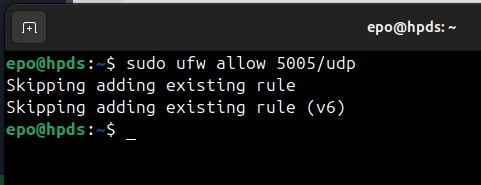
\includegraphics[width=0.85\textwidth]{ImagesPhase2/openPort.png}
    \caption{داشبورد وب پس از باز شدن پورت فایروال و اتصال موفقیت‌آمیز گره‌ها}
    \label{fig:dashboard}
\end{figure}

\subsection{چالش دوم: اختلاف زمانی دریافت پکت‌ها در سیستم چندنوده \lr{(Timestamp Spread)}}
با اضافه کردن گره دوم و سوم، سرور شروع به ادغام داده‌ها (\lr{Multi-Static Fusion}) کرد اما به دلیل \lr{Clock Drift} میکروکنترلرها و تاخیر متغیر شبکه وای‌فای (\lr{Network Jitter})، خطای زیر مداوم چاپ می‌شد:

\begin{latin}
\begin{lstlisting}
WARN fusion error: Timestamp spread exceeds guard interval 60000 us
\end{lstlisting}
\end{latin}

\paragraph{تحلیل و راهکار:} طبق استانداردهای مخزن \lr{RuView}، از مکانیزم تسهیم زمانی \lr{Time-Division Multiplexing (TDM)} استفاده شد. با تنظیم متغیرهای اسلات زمانی، پنجرهٔ گارد تحمل تاخیر سرور برای ۳ نود افزایش یافت:

\begin{latin}
\begin{lstlisting}[language=bash]
cd ~/Desktop/Amirali/WifiSensing/ruview/v2
WDP_TDM_SLOTS=3 WDP_TDM_SLOT_US=200000 cargo run --release --package wifi-densepose-sensing-server -- \
  --udp-bind 0.0.0.0 \
  --udp-insecure-lan \
  --source esp32
\end{lstlisting}
\end{latin}

\subsection{چالش سوم: عبور امواج از دیوار و خطای شناسایی افراد خارج از اتاق}
به‌دلیل خاصیت نفوذ امواج ۲.۴ گیگاهرتز از موانع گچی و شیشه‌ای (\lr{Through-Wall Propagation})، تردد افراد در راهرو مجاور نیز باعث نوسان فاز و افزایش خطای شمارش افراد می‌شد.

\paragraph{راهکار:} برای حذف نویزهای ناشی از عبور از دیوار و متمرکز کردن ناحیه شناسایی بر داخل خود اتاق، آستانه حساسیت به تحرک (\lr{Motion Threshold}) از طریق سرور بالاتر برده شد:

\begin{latin}
\begin{lstlisting}[language=bash]
WDP_TDM_SLOTS=3 WDP_TDM_SLOT_US=200000 WDP_MOTION_THRESHOLD=1.5 cargo run --release --package wifi-densepose-sensing-server -- \
  --udp-bind 0.0.0.0 \
  --udp-insecure-lan \
  --source esp32
\end{lstlisting}
\end{latin}

با اعمال این ضریب، سیگنال‌های تضعیف‌شده ناشی از انعکاس دیوارهای خارجی فیلتر شده و شمارش و حضور پایدار گردید.

\section{نتیجه‌گیری}
در نهایت، با پیکربندی دقیق ۳ گره \lr{ESP32-S3}، تنظیم دسترسی‌های لایه شبکه، همگام‌سازی زمانی پکت‌ها با اسلات‌های \lr{TDM} و بهینه‌سازی آستانه نویز، سیستم مش چندنوده \lr{RuView} با موفقیت به صورت بلادرنگ راه‌اندازی و تثبیت گردید.


\section{روش نوین پیکربندی گره‌ها با استفاده از اسکریپت Provision.py}

پس از آشنایی با روش سنتی پیکربندی از طریق \lr{menuconfig} و کامپایل دستی، در ادامه به سراغ روش کارآمدتر و سریع‌تر رفتیم که امکان تغییر تنظیمات گره‌ها را بدون نیاز به کامپایل مجدد فراهم می‌کند. این روش مبتنی بر نوشتن مستقیم تنظیمات در پارتیشن \lr{NVS (Non-Volatile Storage)} گره‌های \lr{ESP32-S3} است و مزیت‌های قابل‌توجهی از جمله سرعت بالا و عدم نیاز به کامپایل مجدد فریم‌ورک را به همراه دارد.

\subsection{مراحل گام‌به‌گام پیکربندی با اسکریپت Provision.py}

\subsubsection{گام اول: راه‌اندازی محیط و اتصال گره}

ابتدا محیط توسعه \lr{ESP-IDF} را فعال کرده و یک گره \lr{ESP32-S3} را از طریق کابل \lr{USB} به سیستم متصل می‌کنیم. برای اطمینان از شناسایی پورت سریال، دستور زیر را اجرا می‌کنیم:

\begin{latin}
\begin{lstlisting}[language=bash]
. $HOME/esp/esp-idf/export.sh
ls /dev/ttyACM*
\end{lstlisting}
\end{latin}

پس از شناسایی پورت (به عنوان مثال \lr{/dev/ttyACM0})، دسترسی سریال را با دستور زیر فعال می‌کنیم:

\begin{latin}
\begin{lstlisting}[language=bash]
sudo chmod 666 /dev/ttyACM0
\end{lstlisting}
\end{latin}

\subsubsection{گام دوم: تنظیم معماری و پاک‌سازی حافظه فلش}

در این مرحله، هدف معماری (\lr{Target}) را روی \lr{esp32s3} تنظیم کرده و برای جلوگیری از تداخل فریم‌ورک‌های قبلی، حافظه فلش را پاک می‌کنیم:

\begin{latin}
\begin{lstlisting}[language=bash]
cd ~/Desktop/Amirali/WifiSensing/ruview/firmware/esp32-csi-node
idf.py set-target esp32s3
idf.py -p /dev/ttyACM0 erase-flash
\end{lstlisting}
\end{latin}

\subsubsection{گام سوم: فلش فریم‌ورک اصلی}

پس از پاک‌سازی، فریم‌ورک اصلی پروژه را روی گره فلش می‌کنیم. توجه داشته باشید که این فریم‌ورک شامل قابلیت‌های جدید ارسال بسته‌های همگام‌سازی (\lr{Sync Packets}) و پشتیبانی از \lr{ESP-NOW} برای هماهنگ‌سازی زمانی است که در نسخه \lr{v0.8.4} پیاده‌سازی شده است:

\begin{latin}
\begin{lstlisting}[language=bash]
idf.py -p /dev/ttyACM0 flash
\end{lstlisting}
\end{latin}

پس از اتمام فلش، گره را با فشار دادن دکمه \lr{RST} ریستارت می‌کنیم.

\subsubsection{گام چهارم: پیکربندی تنظیمات با اسکریپت Provision.py}

در این مرحله، به جای استفاده از \lr{menuconfig} و کامپایل مجدد، از اسکریپت \lr{provision.py} برای نوشتن مستقیم تنظیمات در پارتیشن \lr{NVS} استفاده می‌کنیم. این اسکریپت اطلاعاتی مانند \lr{SSID}، رمز عبور، آی‌پی سرور، شناسه گره و تنظیمات \lr{TDM} را روی گره ذخیره می‌کند.

برای اولین گره (به عنوان مثال گره شماره ۱)، دستور زیر را اجرا می‌کنیم:

\begin{latin}
\begin{lstlisting}[language=bash]
python provision.py --port /dev/ttyACM0
--ssid "Sharif-WiFi"
--password ""
--target-ip 172.27.2.87
--node-id 1
--tdm-slot 0
--tdm-total 3
\end{lstlisting}
\end{latin}

پس از اجرای دستور، خروجی مشابه زیر مشاهده می‌شود:

\begin{latin}
\begin{lstlisting}
Building NVS configuration:
WiFi SSID: Sharif-WiFi
WiFi Password: (empty)
Target IP: 172.27.2.87
Target Port: 5005
Node ID: 1
TDM Slot: 0 of 3
Flashing NVS partition (24576 bytes) to /dev/ttyACM0...
NVS provisioning complete!
\end{lstlisting}
\end{latin}

این فرآیند در کمتر از یک ثانیه انجام می‌شود و نیازی به کامپایل مجدد نیست.

\subsection{پیکربندی گره‌های بعدی در شبکه مش}

برای افزودن گره‌های بعدی به شبکه مش، مراحل بالا را تکرار می‌کنیم با این تفاوت که پارامترهای \lr{--node-id} و \lr{--tdm-slot} را برای هر گره به‌صورت منحصربه‌فرد تنظیم می‌کنیم.

\subsubsection{گره شماره ۲ (اسلات ۱)}

پس از اتصال گره دوم (که ممکن است روی پورت \lr{/dev/ttyACM1} شناسایی شود)، دستور زیر را اجرا می‌کنیم:

\begin{latin}
\begin{lstlisting}[language=bash]
python provision.py --port /dev/ttyACM1
--ssid "Sharif-WiFi"
--password ""
--target-ip 172.27.2.87
--node-id 2
--tdm-slot 1
--tdm-total 3
\end{lstlisting}
\end{latin}

\subsubsection{گره شماره ۳ (اسلات ۲)}

به همین ترتیب برای گره سوم:

\begin{latin}
\begin{lstlisting}[language=bash]
python provision.py --port /dev/ttyACM2
--ssid "Sharif-WiFi"
--password ""
--target-ip 172.27.2.87
--node-id 3
--tdm-slot 2
--tdm-total 3
\end{lstlisting}
\end{latin}

\subsection{مزایای روش Provision.py نسبت به روش سنتی}

\begin{itemize}
\item \textbf{سرعت بالا:} پیکربندی هر گره در کمتر از یک ثانیه انجام می‌شود.
\item \textbf{عدم نیاز به کامپایل مجدد:} تغییر تنظیمات بدون نیاز به کامپایل مجدد فریم‌ورک امکان‌پذیر است.
\item \textbf{قابلیت تغییر پویا:} امکان تغییر تنظیمات شبکه و مش در هر زمان بدون نیاز به فلش مجدد.
\item \textbf{یکپارچگی با نسخه‌های جدید فریم‌ورک:} پشتیبانی کامل از قابلیت‌های هماهنگ‌سازی زمانی در نسخه \lr{v0.8.4}.
\end{itemize}

\subsection{نکته مهم در خصوص شناسایی پورت گره‌ها}

در صورتی که چند گره به سیستم متصل باشند، برای شناسایی پورت هر گره از دستور زیر استفاده می‌کنیم:

\begin{latin}
\begin{lstlisting}[language=bash]
ls /dev/ttyACM*
\end{lstlisting}
\end{latin}

خروجی این دستور لیستی از پورت‌های فعال را نمایش می‌دهد که می‌توانیم با اتصال و قطع هر گره، پورت متناظر با آن را شناسایی کنیم.

\subsection{اجرای سرور با تنظیمات بهینه}

پس از پیکربندی تمام گره‌ها، سرور را با تنظیمات بهینه برای شبکه مش ۳ گره‌ای اجرا می‌کنیم:

\begin{latin}
\begin{lstlisting}[language=bash]
cd ~/Desktop/Amirali/WifiSensing/ruview/v2
WDP_GUARD_INTERVAL_US=150000 cargo run --release --package wifi-densepose-sensing-server --
--source esp32
--udp-port 5005
--udp-bind 0.0.0.0
--udp-insecure-lan
--http-port 3000
--ws-port 3001
--ui-path ../ui
\end{lstlisting}
\end{latin}

با این روش، سیستم مش چندگره‌ای با موفقیت راه‌اندازی شده و داده‌های \lr{CSI} از هر سه گره به‌صورت هماهنگ دریافت و پردازش می‌شوند.

\appendix
\section{پیوست‌ها و دستورات کمکی شبکه و سخت‌افزار}

\subsection{شناسایی پورت سریال گره متصل‌شده \lr{(Port Detection)}}
برای تشخیص نام پورت اتصالی گره‌های \lr{ESP32-S3} به سیستم اوبونتو، می‌توان از دستورات زیر استفاده کرد:

\paragraph{روش اول (بررسی سریع پورت‌های مدرن):}
بررسی میکند کدام پورت ها اشغال هستند.

\begin{latin}
\begin{lstlisting}[language=bash]
ls /dev/ttyACM*
\end{lstlisting}
\end{latin}

\paragraph{روش دوم (مانیتورینگ رویدادهای زنده هسته لینوکس):}
بلافاصله پس از اتصال کابل \lr{USB}، دستور زیر پورت شناسایی‌شده را چاپ می‌کند:

\begin{latin}
\begin{lstlisting}[language=bash]
dmesg | grep -i "tty" | tail -n 5
\end{lstlisting}
\end{latin}

\subsection{استخراج آدرس IP کامپیوتر مقصد \lr{(Aggregator IP)}}
برای پیدا کردن آدرس \lr{IP} محلی لپ‌تاپ جهت تنظیم در منوی \lr{menuconfig} گره‌ها:

\begin{latin}
\begin{lstlisting}[language=bash]
hostname -I | awk '{print $1}'
\end{lstlisting}
\end{latin}

\subsection{تغییر IP پس از ری‌استارت و راه‌حل تثبیت آن \lr{(Static IP)}}
\paragraph{پرسش:} در صورت اتصال با کابل \lr{LAN} و خاموش/روشن شدن سیستم، آیا \lr{IP} تغییر می‌کند و نیاز به پروگرام مجدد بردهاست؟

\paragraph{پاسخ و تحلیل:} بله؛ در صورتی که کارت شبکه روی حالت \lr{DHCP} (دریافت خودکار \lr{IP}) تنظیم شده باشد، روتر شبکه ممکن است پس از ری‌استارت یک \lr{IP} جدید اختصاص دهد. در این حالت پکت‌های ارسالی بردها به مقصد قبلی می‌روند و سرور چیزی دریافت نمی‌کند.

\paragraph{پیشنهاد:}
در صورت روشن و خاموش شدن مجدد کامپیوتر ممکن است نیاز به پروگرم کردن مجدد esp32 
ها با IP 
جدید است.

\end{document}